% !TEX encoding = UTF-8 Unicode
% ÄÖÜ ß äöü

\section{Architecture}

The general design of \Nyaya follows the Model-View-Controller pattern,
which is originated in Smalltalk \cite[p.4]{GAMMAETAL}, 
that separates the representation of data from the user interaction.
Cocoa Touch (see \vref{sec:Cocoa}) encourages the use of MVC 
by providing a rich set of useful views and controllers with the framework UIKit.
These cover many use cases of data presentation and user interaction.

\section{Model}

\Nyaya must hold different representations of Boolean functions – propositional formulas, abstract syntax trees and binary decision diagrams. 

\subsection{Propositional formulas and Boolean expressions}
Since propositional formulas and Boolean expressions are subsets of the set of all Unicode strings,
they are easily represented by the standard string classes of actual frameworks. 

Due to the unambiguous relationship between propositional formulas and Boolean expressions 
\Nyaya allows the use of a mixed syntax and additional symbols as input
for the user's convenience. The input expression $!a \wedge b + c \oplus a$ translates into the propositional formula
$\neg a \wedge b \vee c \veebar a$ (see \vref{subsec:Parser}).

\subsection{Abstract Syntax Trees}

Cocoa does not provide a class to represent trees, 
but with instances of a class, 
that implements the composite pattern \cite[p.163ff]{GAMMAETAL}
arbitrary graphs and therefore syntax trees can be represented easily.

\begin{figure}[htbp]
\begin{center}
\UML{NyayaNode.png}
\caption{Node class to represent an abstract syntax tree}
\label{fig:NyayaNodeCluster}
\end{center}
\end{figure}

\subsubsection{Node class cluster}

The node class is implemented as a class cluster, 
which is a Cocoa design pattern \cite[p.282ff]{Buck:2009:CDP:1803585}
– an adaptation of the the abstract factory design pattern \cite[p.87ff]{GAMMAETAL}.
The abstract and public class \verb+NyayaNode+ 
provides a set of static and public methods (see \figref{fig:NyayaNodeCreation}),
that returns instances of non public sub-classes (see \figref{fig:NyayaNodeCluster})
of \verb+NyayaNode+.

\begin{figure}[htbp]
\begin{center}
\UML{NyayaNodeCluster.png}
\caption{Public root class and non public subclasses}
\label{fig:NyayaNodeCluster}
\end{center}
\end{figure}

Actually the creational methods were implemented as a class category in a different source file. 
Class categories are a language feature of Objective-C \cite[p.225ff]{Kochan:2009:PO:1538451}
– an adaptation of the decorator design pattern \cite[p.175ff]{GAMMAETAL} – 
to extend or organize the functionality of given classes beyond their core purpose. 

There are base implementations of category methods in the root node class,
that will be overridden in subclasses.
For example \verb+isLiteral:bool+ returns false for all node instances
except for instances of variables
and instances of negations of variables.

The variable node class adds setters for the categories \verb+Valuation+  (\figref{fig:NyayaNodeValuation})
and \verb+Display+.

\subsubsection{Node class categories}

\begin{itemize}

\item The category “Creation” implements the production rules of the grammar 
to create syntax trees recursively (\figref{fig:NyayaNodeCreation}).
Since the constructors of all classes in the cluster are hidden, 
the production of invalid syntax trees is prevented.

\begin{figure}[htbp]
\begin{center}
\UML{NyayaNodeCreation.png}
\caption{Production rules}
\label{fig:NyayaNodeCreation}
\end{center}
\end{figure}

\item The category “Description” provides methods to convert a syntax tree into one of it's string representations – 
either a propositional formula in strict syntax with many parentheses 
or a formula using precedences and associativity.
In most cases, the second form leads to shorter strings with less parentheses. 
In rare case, only the outer parentheses are omitted.

\item The category “Display”  allows extended valuations (undefined, false, true) 
with incomplete truth assignments. 
It is used for the interactive syntax tree view on the playground, 
where the user can assign truth values to some or all atoms.
% (see \figref{fig:NyayaNodeDisplay)


\item The category “Attributes”  provides information about the number of sub-nodes of a node 
and the normal forms the sub-tree matches.

\item The category “Transformations” provides equivalence transformations 
and methods to create 
 semantically different syntax trees by replacing atoms, connectives or sub-trees with
atoms, connectives or trees.

\item The category “Derivations” defines methods to derive semantically equivalent normal forms from a given syntax tree.

\item The category “Random” creates arbitrary syntax trees with a given set of connectives and atoms and within a range for the number of nodes. It is used to create formulas for the exercises.

%\item The category “Reductions”
%\item The category “Resolution”
\item The  category “Type” provides a method, 
that returns the type of a node, i.e constant, variable, type of connective as an enum.


\item The category “Valuation” (\figref{fig:NyayaNodeValuation}) 
provides fast valuations with complete truth assignments. 
It is used to create truth tables and binary decision diagrams. 

\begin{figure}[htbp]
\begin{center}
\UML{NyayaNodeValuation.png}
\caption{Valuation of trees}
\label{fig:NyayaNodeValuation}
\end{center}
\end{figure}

\end{itemize}
\subsubsection{Immutable syntax trees}

Instances of node classes are not mutable 
regarding their function as nodes of abstract syntax trees. 
This means nodes can be created, but not modified.
The symbol of an atom can not be changed, 
a connective node can not be altered into another one,
and child nodes of a connective node can not be replaced or reordered.

Derivations or transformations do not change the structure of an existing syntax tree,
but rather create a new independent syntax tree.

Obviously mutable truth assignments do not affect the immutable structure of a syntax tree,
because truth assignments are semantics, not syntax. 

\subsubsection{Acyclic syntax graphs}

Since the representation of abstract syntax trees is implemented immutable,
there is no need to create multiple instances for syntactically equivalent sub-trees. 
At run-time syntax trees are represented by acyclic syntax graphs, 
where multiple sub-trees can be represented by the same instance-graph
(\figref{fig:AST+ASG}).

\begin{figure}[htb]
\begin{center}
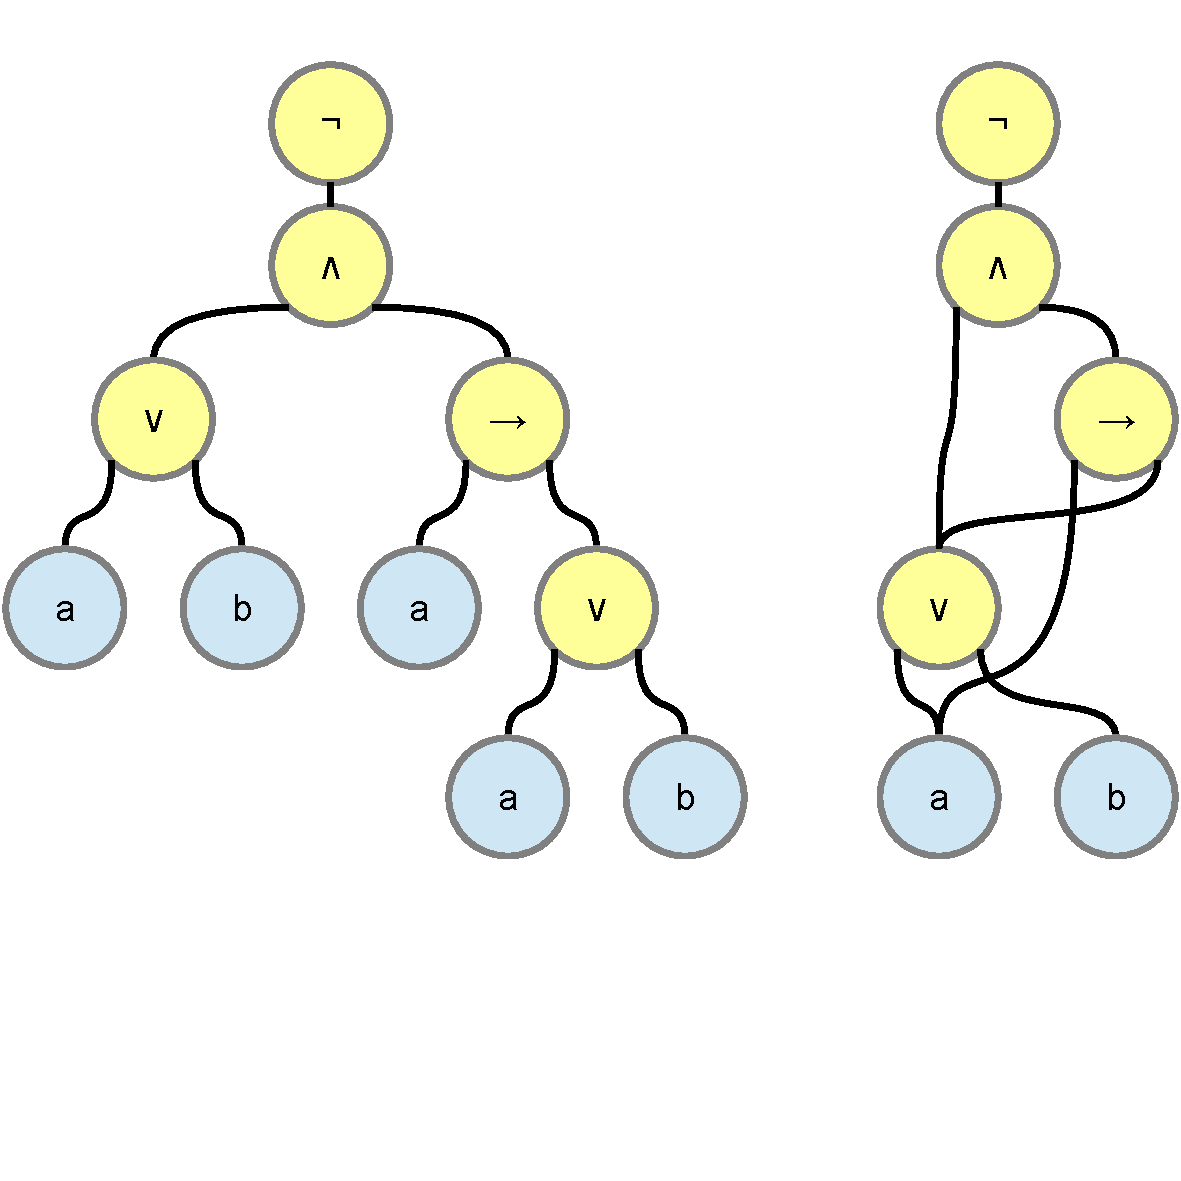
\includegraphics[scale=0.5,trim=0cm 5.4cm 0cm 1cm,clip=true]{diagrams/AcyclicSyntaxGraph.pdf}
\caption{Abstract syntax tree – acyclic graph }{$\neg( (a\vee b) \wedge (a \rightarrow a\vee b))$}
\label{fig:AST+ASG}
\end{center}
\end{figure}

This eases the detection of obvious tautologies $P \vee \neg P$, $P \rightarrow P$ and contradictions $P \wedge \neg P$,
because the sub-tree $P$ on the left side is represented by the same object-graph as the sub-tree $P$ on the right side.

\subsubsection{Limitations}

The derivation of normal forms will fail on some relatively small syntax trees.
especially when the formula contains too many exclusive disjunctions.

With every exclusive disjunction of a formula $P$ and an atom $p$, 
that is not already used in $P$,
the number of nodes will at least double 
when deriving an equivalent implication free form.
“Implication free” means also the absence of exclusive disjunctions (see \tabref{tab:BNFGRIFF}).

\begin{eqnarray*}
\#(P \oplus p) & = & 1 \cdot(\#(P) + 2) \\
\#((P \wedge \neg p) \vee  (\neg P \wedge p)) & = & 2 \cdot (\#(P) + 2) + 3 \\
\#((P \vee p) \wedge  (\neg P \vee \neg p)) & = & 2 \cdot (\#(P) + 2) + 3 \\
\end{eqnarray*}

The syntax tree for an exclusive disjunction of 20 different atoms is build from 39 nodes.
The syntax tree of a semantically equivalent implication free form will already contain over four million nodes.
Deriving the negation normal form does not increase or decrease the number of nodes significantly,
but the necessary distributions of disjunctions will multiply the number of nodes again.

To ensure the stability of \Nyaya 
and since it is near impossible 
to present a propositional formula 
with thousands of symbols 
in a meaningful way
to the user, 
the derivation of normal forms is aborted, when the results surpass a defined size.



\subsection{Parser}
\label{subsec:Parser}

The backend of \verb+BoolTool+\footnote{
\href{http://cl-informatik.uibk.ac.at/software/booltool/}{cl-informatik.uibk.ac.at/software/booltool/}} 
– parsing and transformation of Boolean functions – 
is implemented in \verb+OCaml+\footnote{
\href{http://ocaml.org}{ocaml.org}}, 
a functional programming language, which is well suited for this kind of task.

After several failed attempts to cross-compile the \verb+OCaml+ sources to iPad's processor architecture (ARM),
to link the object code to the Xcode project and to bridge and call functions from C, 
the implementation of a simple translator 
for propositional formulas (a subset of all possible strings)
into syntax trees looked more promising. 

The generation of a syntax tree from a formula  is carried out in two steps. 

\subsubsection{Scanning}

In the first step the input string is transformed into an array of strings – the list of input tokens –
using the standard regular expression class of Cocoa Foundation.
\begin{table}[htdp]
\begin{center}
$\top | \bot 
| \neg | !
| \wedge | \& | .
| \vee | {\setminus}| | {\setminus}+ 
| \veebar | \oplus | \textasciicircum
| = | <> | \leftrightarrow 
| > | \rightarrow | \models
| ( | ) | , | ; 
| {\setminus}w+$ 
\caption{Regular expression for the scanner}
\label{tab:REGEX}
\end{center}
\end{table}

The set of valid tokens, which includes identifiers, connectives and parentheses
was simply defined by writing a suitable regular expression (see \tabref{tab:REGEX}), 

\subsubsection{Parsing}

In the second step the list of input tokens is parsed top-down 
using a recursive-descent parsing algorithm \cite[p.144ff]{Louden:1997:CCP:523017} 
following an ebnf grammar outlined in \tabref{tab:CoreEBNF}), 
that defines precedence and associativity of connectives too.

\begin{table}[htdp]
\begin{center}
\begin{lstlisting}[mathescape]
formula        ::= entailment
entailment     ::= sequence [ '$\models$' entailment]
sequence       ::= bicondition { ';' bicondition } 
bicondition    ::= implication [ '$\leftrightarrow$' bicondition ]
implication    ::= xdisjunction [ '$ \rightarrow$' implication ]
xdisjunction   ::= disjunction { '$\veebar$' disjunction }
disjunction    ::= conjunction { '$\vee$' conjunction }
conjunction    ::= negation { '$\wedge$' negation }
negation       ::= '$\neg$' negation | '(' formula ')' | identifier
\end{lstlisting}
\caption{Core EBNF grammar for the parser}
\label{tab:CoreEBNF}
\end{center}
\end{table}

\subsubsection{Limitations}

\Nyaya does not parse as fast and (memory) efficient as BoolTool's parser,
primarily because recursion and token probing are more expansive operations in Objective-C than in OCaml.
The creation of a syntax graph instead of a syntax tree adds more overhead.
But \Nyaya's implementation is {\em good enough}, 
because {\em real world} user input is limited to at most a few thousands characters.

The unit tests have shown that there are no memory or run-time issues, 
although the parsing can take a second or two on an iPad.

\subsubsection{Enhancements}

Despite the drawbacks mentioned above
the benefits far outweigh the disadvantages of implementing its own parser.

\begin{itemize}

\item \Nyaya parses strings with Unicode characters, 
therefore identifiers are not limited to Latin letters and
$\alpha + \omega$ will be parsed correctly. 

\item The grammar rules for operators are defined as sets of tokens, 
which will be initialized at application start. 

\begin{table}[htdp]
\begin{center}
\begin{lstlisting}[mathescape,firstnumber=7]
disjunction    ::= conjunction { OR conjunction }
\end{lstlisting}
\begin{lstlisting}[mathescape,firstnumber=15]
OR             ::= '$\vee$' | '$|$' | '$+$' | 'O'
\end{lstlisting}
\caption{Excerpts from a localized grammar (Italian)}
\label{tab:LocalizedEBNF}
\end{center}
\end{table}
% conjunction    ::= negation { AND negation }
% AND            ::= '$\wedge$' | '$.$' | '$\&$' | 'E'

\item Symbols for operators
can be localized using the standard localization framework of Cocoa.

\begin{table}[htdp]
\begin{center}
\begin{lstlisting}[mathescape,numbers=none,multicols=2]
IMP = "$\rightarrow$ $>$ IMPLIES";
OR  = "$\vee$ | + OR";
AND = "$\wedge$ & . AND";
NEG = "$\neg$ ! ~ NOT";
IMP = "$\rightarrow$ $>$ IMPLICA";
OR  = "$\vee$ | + O";
AND = "$\wedge$ & . E";
NEG = "$\neg$ ! ~ NON";
\end{lstlisting}
\caption{Localizable.strings in en.lproj and it.lproj}
\label{tab:LocalizableStrings}
\end{center}
\end{table}


\item The parser generates syntax graphs with Objective-C run-time objects,
which are well suited for the use cases in an interactive environment.

\end{itemize}

\subsection{Truth Tables}

Truth tables are either small enough to be computed on demand or too big to be stored in memory.
Either way there is no reason to store filled truth tables at run-time.

\subsection{Binary Decision Diagrams}

Binary decision trees and diagrams are represented by trees 
or acyclic directed graphs built from instances of a simple node class
 with attributes for a name, a left branch and a right branch. 
\begin{table}[htdp]
\begin{center}
\UML{BddNode.png}
\caption{Attributes and factory method of BddNode}
\label{fig:BddNode}
\end{center}
\end{table}
The name is either an identifier, i.e. the name of a variable, “0” or “1". 
Nodes with the name “0” or “1” are leaf nodes or result nodes
and must not have a left or right branch.
The other nodes with the name of a variable are decision nodes 
and must have valid left and right branches. 

The class provides a factory method to create 
(un)reduced ordered binary decision diagrams from abstract syntax trees
(\figref{fig:BddNode}).

\newpage\section{Views and Controllers}

\Nyaya's main navigation – switching between Welcome, Tutorials, Playground, Glossary and NyBoolTool – 
is organized by a sub-class of\verb+ UITabBarController+ (an heir of \verb+UIViewController+). 
At start the tab bar controller will be instantiated and invoked by \Nyaya's application delegate. 
The tab bar controller will present it's \verb+UITabBar+ (an heir of \verb+UIView+)
and will appoint of one of its view controllers, which will present its view such as the welcome screen.

Tabbing an \verb+UITabBarItem+ will cause the tab bar to delegate the event to its \verb+UITabBarDelegate+ – the tab bar controller.
The tab bar controller will switch the selected view controller, which then will present its content.

Except for the welcome view controller 
all content view controllers inherits from split view controller,
which provides a master view controller and a detail view controller.
The tutorial master view controller and the BoolTool master view controller shares a list of persisted formulas.

\subsection{Welcome}

The welcome view controller is a simple subclass of\verb+ UIViewController+ 
and presents its content in a not so simple \verb+UIWebView+,
which is a fully functional, but ‘naked’ web-browser, i.e. links are followed and there is a page history, but no back-button is presented.
The behavior of the web view can be altered by implementing a web view delegate – usually the controller.

\subsection{Tutorials}

The tutorials master view controller presents a table view with five sections of tutorials.
The sections organize the tutorial titles for 
introduction, syntax, semantics, normal forms and binary decision diagrams.
Tabbing an entry will cause the detail view controller to present the corresponding tutorial in a web view
with an additional exercise button on the top of the view.

Tabbing this exercise button will put the exercise view controller in charge. 
A suitable overlay view will be opened, 
and an instance of a matched class implementing of\verb+ NyTuTester+ will be created.

\begin{figure}[htbp]
\begin{center}
\UML{NyTuTester.png}
\caption{Tester interface}
\label{fig:Tester}
\end{center}
\end{figure}

The method \verb+firstTest+ initializes the test parameters and fills the test view with instructions and labels. 
Then it calls \verb+nextTest+, which will fill the test view with a new question with every call.
The method \verb+checkTest+ evaluates the user's answer and displays the result in the test view.
When the test view is closed by the user \verb+removeTest+ will dispose resources attached to the test view.

\subsection{Playground}

The playground master view controller presents a table view with the list of stored and selectable formulas.
The user can use a formula from this list to add a tree view to the detail view – the canvas view.
Or the user can add a new tree view to the canvas view using a tap and hold gesture.
The canvas view can hold multiple syntax trees.

\begin{figure}[htbp]
\begin{center}
\UML{TreeView.png}
\caption{Canvas view with multiple syntax tree views}
\label{fig:TreeView}
\end{center}
\end{figure}

The nodes of the syntax tree view are drawn as circles around the \verb+symbol()+ 
method defined in the category
\verb+Display+ of the class \verb+NyayaNode+.
The color of the border is determined by the value of \verb+displayValue()+.


\begin{figure}[htbp]
\begin{center}
\UML{NyayaNodeDisplay.png}
\caption{Node display interface}
\label{fig:NyayaNodeDisplay}
\end{center}
\end{figure}

\subsection{Glossary}

The glossary master view controller reads all elements with an id from the glossary content document,
creates an alphabetically ordered list of technical terms using the texts included between the corresponding element-tags.
This list of technical terms defined by the glossary document is presented in a table view.
Tapping a term will scroll the glossary document view – a web view - to the chosen term, 
controlled by the glossary detail view controller.

\subsection{BoolTool}

The BoolTool master view controller presents a table view with stored and selectable formulas.
An editable text field with an attached customized keyboard will allow the user to enter their formulas.

The output will be presented in different views. Read only text views are used for the normal form, 
a web form is used for the truth table and a customized view will draw the binary decision diagram.



%\section{Unit-Tests}
%\newpage
\section{Application content}

Beside the classes to determines the run-time behavior of the application,
the storage of application content must be defined.

\subsection{Content on delivery}

Configuration data, localization data and html documents
are stored in UTF-8 encoded text files.
All graphical content such as icons and diagrams are stored in portable network graphics.
These content files are embedded in \Nyaya's app bundle
and will be downloaded along the application execution data,
while receiving \Nyaya for iPad from the App Store.

\subsection{User created content}

Formulas from the playground and BoolTool are persisted 
in the simple property list file \verb+BoolToolData+ 
in the documents folder of the app.

\subsection{Export and import of content}

Single formulas can be exported from or imported into editable text fields 
by simply using the standard copy and paste mechanism of iOS.




